\documentclass[10pt,a4paper,oneside]{article}
\usepackage[utf8]{inputenc}
\usepackage{amsmath}
\usepackage{amsfonts}
\usepackage{amssymb}
\usepackage{graphicx}
\usepackage{draftwatermark} % 设置水印
\SetWatermarkText{DNV Group} % 水印内容
\usepackage{breqn}
\usepackage{tikz} % system block diagram
\usepackage{textcomp}
\usetikzlibrary{datavisualization}
\usetikzlibrary{shapes,arrows} % system block diagram
\usepackage{booktabs}
\usepackage[framed,numbered,autolinebreaks,useliterate]{mcode} % matlab code block
\author{Yangang Cao}
\date{February 26, 2019}
\newcommand{\degree}{^\circ}
\tikzset{
	delay/.style    = {draw, thick, rectangle, minimum height = 3em,
		minimum width = 3em},
	sum/.style      = {draw, circle, node distance = 2cm}, 
	prod/.style     = {draw, circle, node distance = 2cm},
	input/.style    = {coordinate}, % Input
	output/.style  = {coordinate} % Output
}
% Defining string as labels of certain blocks.
\newcommand{\product}{$\displaystyle \times$}
\newcommand{\delay}{\large$z^{-1}$}
\begin{document}

\title{Limiter}
\maketitle 
The limiter is used to control the highest peaks in the signal, but to otherwise change the dynamics of the signal as little as possible. Limiting can refer to a range of treatments designed to limit the maximum level of a signal. Treatments in order of decreasing severity range from clipping, in which a signal is passed through normally but sheared off when it would normally exceed a certain threshold; soft clipping which squashes peaks instead of shearing them; a hard limiter, a type of variable-gain audio level compression, in which the gain of an amplifier is changed very quickly to prevent the signal from going over a certain amplitude or a soft limiter which reduces maximum output through gain compression, soft limiter is introduced in this documentation.
\begin{center}
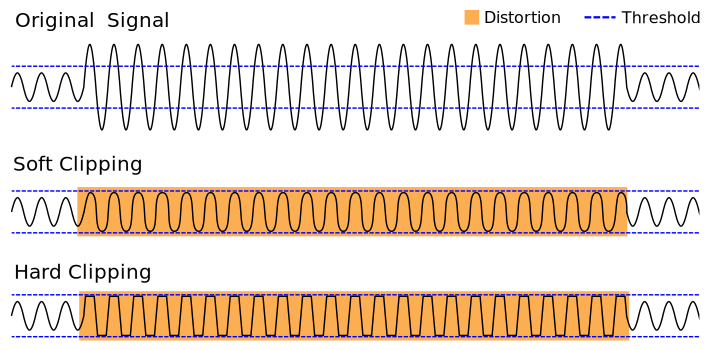
\includegraphics[height=200pt]{Clipping_waveform.eps} 
\end{center}


This is achieved by employing a characteristic curve with an infinite ratio $R = \infty$ above a limiter threshold $LT$(Capital letters represent the logarithmic domain) , i.e.,
\begin{align*}
G &=
\begin{cases} 
0 \ \mbox{dB}  &\mbox{if }X < LT\\
LT-X &\mbox{else}.
\end{cases}
\end{align*}
Thus, the output level $Y = X + G$ should never exceed the threshold $LT$. By lowering the peaks, the overall signal can be boosted. Beside limiting single instrument signals, limiting is also often performed on the final mix of a multichannel application.

A limiter makes use of peak level measurement and should react very quickly when the input signal exceeds the limiter threshold, slowly when belows correspondingly. Typical parameters for a limiter are $t_{AT}$ = 0.02...10 ms and $t_{RT}$ = 1...5000 ms, for both the peak measurement and the smoothing filter. Actually, $t_{AT}$ is far greater than $t_{RT}$, an actual implementation may perform the gain computation in linear values by
\[
g ( n ) = \min \left( 1 , \frac { l t } { x _ { \mathrm { PEAK } } ( n ) } \right),
\]
and block diagram.
\begin{center}
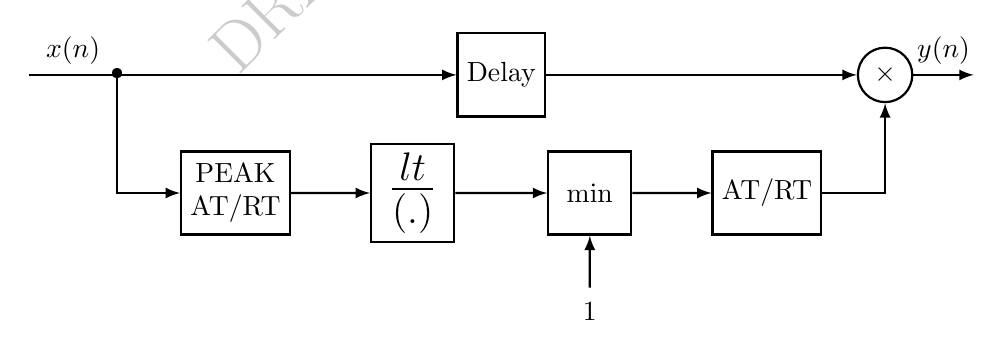
\begin{tikzpicture}[auto, thick, node distance=0.6cm, >=latex, scale = 0.75]
\draw
node at (1,0) {\textbullet}
node at (3,-2) [delay,align=center](d1) {PEAK \\ AT/RT}
node at (6,-2) [delay] (d2){\huge$\frac{lt}{(.)}$}
node at (9,-2) [delay] (d3){min}
node at (12,-2) [delay] (d4){AT/RT}
node at (14,0) [prod] (p1){\product}
node at (7.5,0) [delay] (d5){Delay}
node at (9,-4) {1};

\draw[-](-0.5,0)--node{$x(n)$}(1,0);
\draw[->](1,0)|-(d1);
\draw[->](d1)--(d2);
\draw[->](d2)--(d3);
\draw[->](d3)--(d4);
\draw[->](d4)-|(p1);
\draw[->](1,0)--(d5);
\draw[->](d5)--(p1);
\draw[->](9,-3.6)--(d3);
\draw[->](p1)--node{$y(n)$}(15.5,0);
\end{tikzpicture}
\end{center}
where $lt = 10^{\frac{LT}{20}}$ is the threshold on the linear scale. This approach is also used in following {\bfseries Matlab} code, a very simple limiter implementation with the same filter coefficients in the level detector and the smoothing filter.
\begin{lstlisting}
function y = limiter(audio, para)
% para: threshold of limiter in linear scale (lt)
at = 0.3; % Attack time
rt = 0.01; % Release time
delay = 5;

audiopeak = 0; % intialization
g = 1; % gain
buffer = zeros(1,delay);

for n = 1:length(audio)
	a = abs(audio(n));
	if a > audiopeak
		coeff = at;
	else
		coeff = rt;
	end
	audiopeak = (1-coeff) * audiopeak + coeff * a; % Level detector (A full-wave rectifier in combination with an AR-averager)
	f = min(1, para / audiopeak); %Static curve
	if f < g
		coeff = at;
	else
		coeff = rt;
	end
	g = (1-coeff) * g + coeff * f; % Smoothing filter
	y(n) = g * buffer(end);
	buffer = [audio(n) buffer(1:end-1)];
end
\end{lstlisting}

Limiters are common as a safety device in live sound and broadcast applications to prevent sudden volume peaks from occurring. Limiters are also used as protective features in some components of sound reinforcement systems (e.g., powered mixing boards and power amplifiers) and in some bass amplifiers, to prevent unwanted distortion or loudspeaker damage.
\end{document}
